\documentclass[12pt]{article}
\usepackage{graphicx}

\begin{document}
  
\title{Project 1}
\author{Minh Le}


\section{Effective Sample Size}
\subsection{Computing $\theta$}

In this section, we examine the effectiveness of picking different $g(x)$ to compute $\theta = \int \sqrt{x^2 + y^2}\pi(x,y)dxdy$ 

\begin{itemize}
  \item For $\hat{\theta}_1$, we will draw from $\pi(x,y)$ directly.
  
  \item $\hat{\theta}_2$ will be drawn from g(x,y) a bivariate gaussian with parameters $\mu = (0,0)$ and $\sigma_0 = 1$ We assume independence between x and y.
  
  \item $\hat{\theta}_3$ will be drawn from g(x,y) a bivariate gaussian with parameters $\mu = (0,0)$ and $\sigma_0 = 1$ We assume independence between x and y.
\end{itemize}

Comparing between $\hat{\theta}_2$ and $\hat{\theta}_3$, I believe that $\hat{\theta}_3$ will converge more quickly to $\theta$. This is because both models are drawn from a distribution whose mean is not the true mean $\mu=(2,2)$ meaning the masses of $g$ and $pi$ are not distributed in the same points. It is more likely for us to draw samples close to this the mass of $\pi$ from $g_3$ because of the larger standard deviation.  

We clearly see this when plotting the estimated $\theta$ for different $g$ distributions. We see that $\hat{\theta}_3$ converges to $\hat{\theta}_1$ baseline faster than $\hat{\theta}_2$ as n increases in the log sample plot in the next page.

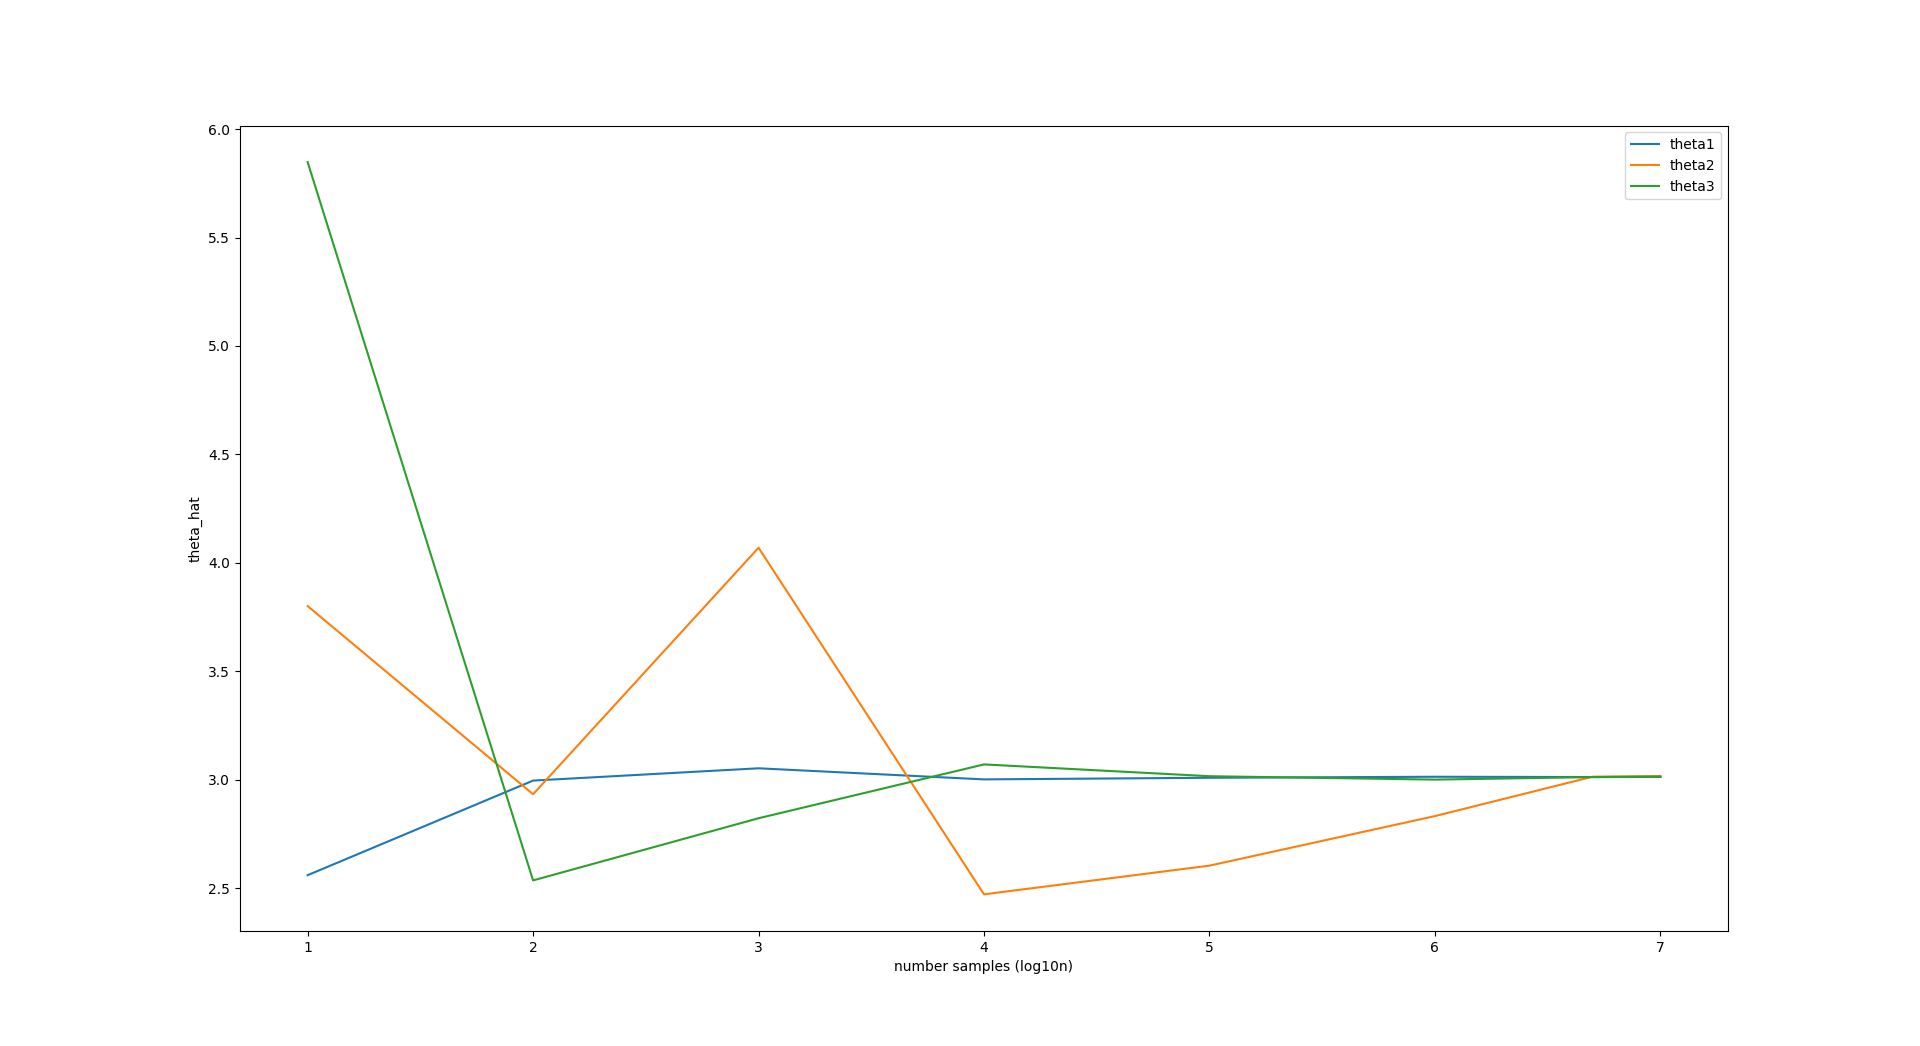
\includegraphics[scale=.25]{problem1_samples}
	
\subsection{effective samples size}
I was unsure on how to interpret the $ess*(n)$ My understanding was that was the $ess$ for the $n_2$ and $n_3$ when $\theta_2$ and $\theta_3$ converged to $\theta_1$. When normalizing $ess$ for $\theta_2$ and $\theta_2$ with the defined $ess*(n_2)$ and $ess*(n_3)$ respectively we saw that the effective sample size of $\theta_3$ increased much faster than $\theta_2$ which furthered my prediction that the former is a better sampler.
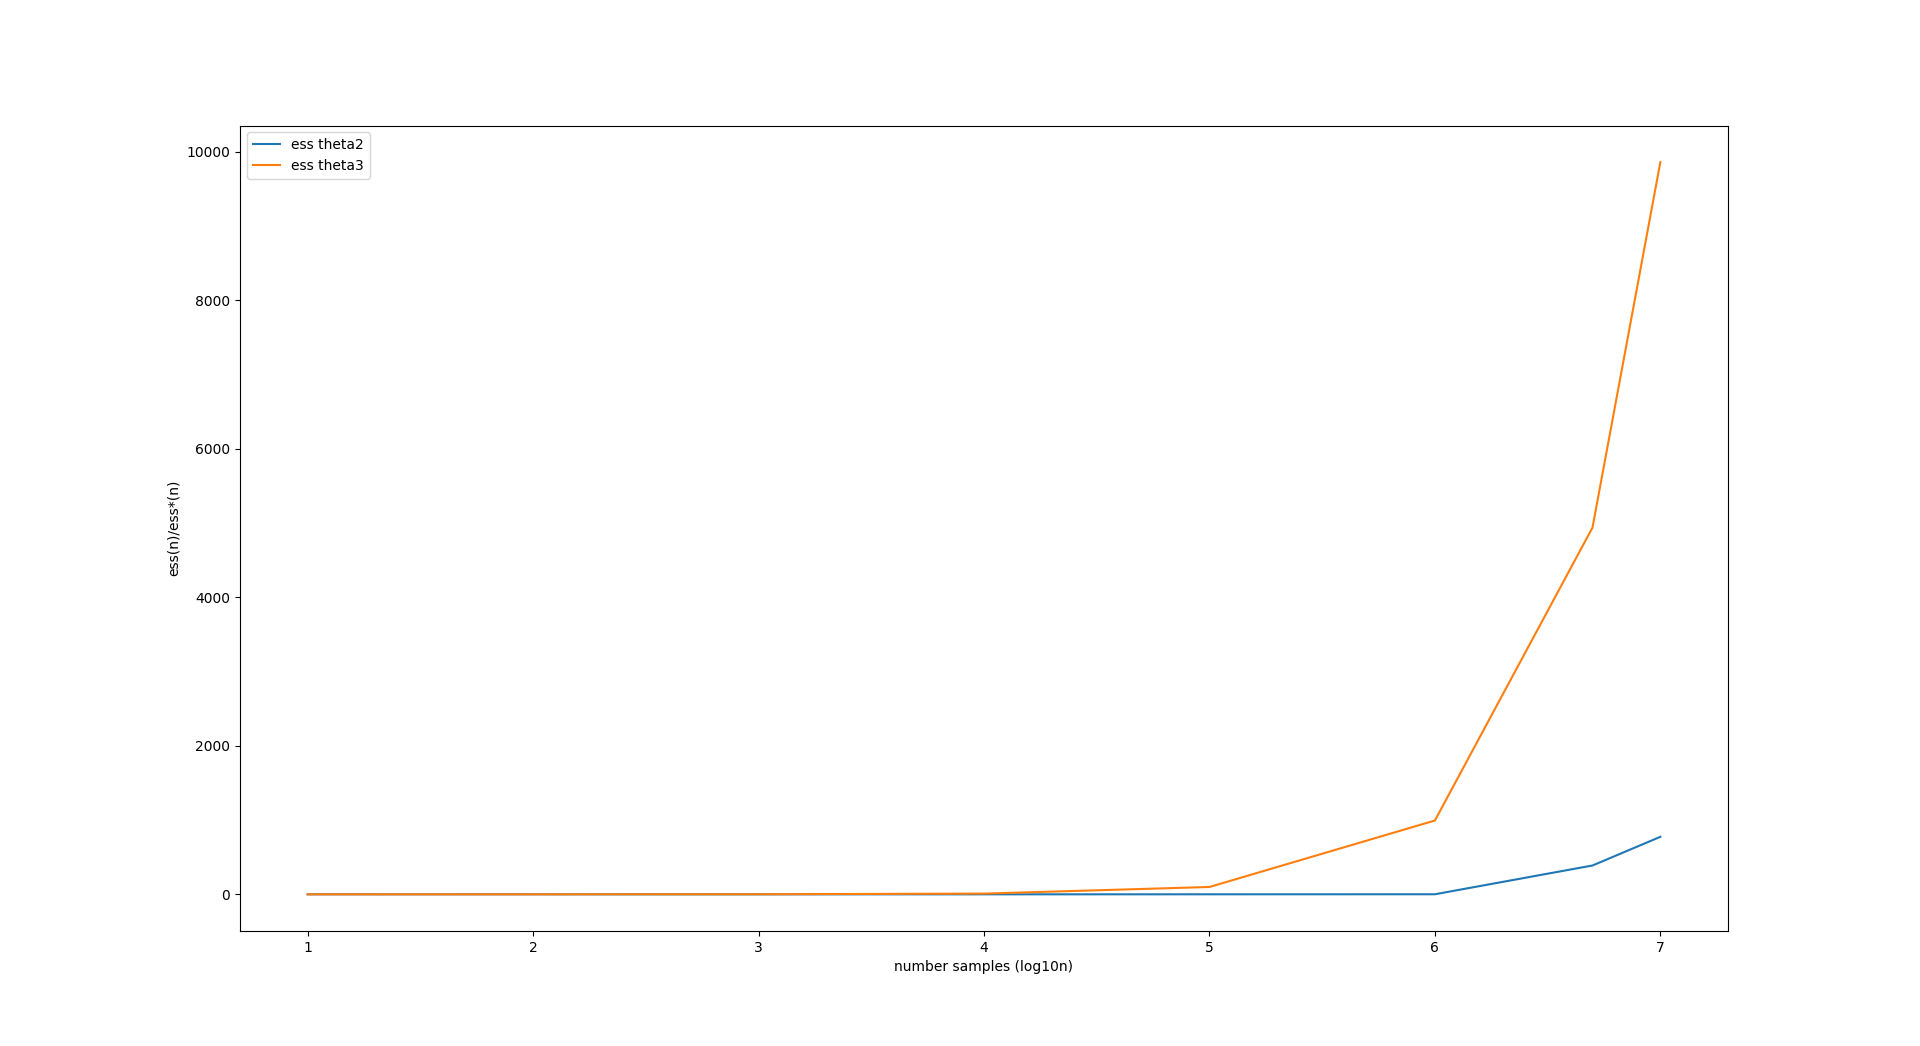
\includegraphics[scale=.25]{ess_1}



\newpage

\section{SAW}
\subsection{Total Number of SAWS}
\begin{itemize}
  \item Design 1 was attempting to d . At $M=10^7$, the estimated number of SAW is 
  
  \item Design 2 accounted for the fact . At $M=10^7$, the estimated number of SAW is 
  
  \item Design 3 was a decaying epsilon so . At $M=10^7$, the estimated number of SAW is 
 
\end{itemize}
We plot the number of estimated SAW's against M. Here we see that 


\subsection{Total Number of SAWS from corner to corner}
Here, I used the same sampling method and P(x) as above except I divided by number of attempts. I also should note that I only recorded paths that ENDED at (n,n) meaning there were no more valid moves. For each method respectively, I got the following
\begin{itemize}
  \item Design 1, at $M=10^7$, the estimated number of SAW is 
  \item Design 2, at $M=10^7$, the estimated number of SAW is 
  \item Design 3, at $M=10^7$, the estimated number of SAW is
\end{itemize} 
\end{document}

